% ========= DOCUMENT =========
\NeedsTeXFormat{LaTeX2e}
\RequirePackage[l2tabu, orthodox]{nag} % checks for obsolete packages and outdated commands, needs to be before documentclass
\documentclass[12pt,a4paper]{article}

\usepackage{titlecaps} % adds \titlecap for title case transformations
% ========= LANGUAGE =========
\usepackage[ngerman,english]{babel} % for different languages
%\DeclareFontShape{OT1}{cmtt}{bx}{n}{<5><6><7><8><9><10><10.95><12><14.4><17.28><20.74><24.88>cmttb10}{} % for bold monospaced font
\usepackage[T1]{fontenc} % output encoding for accented characters
\usepackage[utf8]{inputenc} % input encoding for accented characters by keyboard

\selectlanguage{english}
\newcommand{\iauthor}{Georg Eschbacher BSc.}
\newcommand{\isupervisorone}{Assist.-Prof. Dipl.-Ing. Dr.techn. Marc Streit}
\newcommand{\isupervisortwo}{FH-Prof. DI Dr. Simon Ginzinger, MSc}

\newcommand{\imatrikel}{1410695001}
\newcommand{\ititleone}{Animated Transitions between Geo-Spatial Visualisations}
\newcommand{\ititletwo}{Animated Transitions between \\Geo-Spatial Visualisations}
\newcommand{\ipapertype}{Masterthesis}

%\newcommand{\tattainment}{for attainment of the academic degree}
%\newcommand{\tdegree}{Master of Science}
%\newcommand{\tauthor}{Author}
%\newcommand{\tsubmitted}{Submitted at the master course MultiMediaTechnology, Salzburg University of Applied Sciences}
%\newcommand{\texamined}{Examined by}
%\newcommand{\tsupervisor}{Supervisor}

\newcommand{\tattainment}{zur Erlangung des akademischen Grades}
\newcommand{\tdegree}{Master of Science}
\newcommand{\tauthor}{Verfasser}
\newcommand{\tsubmitted}{Vorgelegt am FH Masterstudiengang MultiMediaTechnology, Fachhochschule Salzburg}
\newcommand{\texamined}{Begutachtet durch}
\newcommand{\tsupervisor}{Betreuer}

\title{\ititle}
\author{\iauthor}


%\usepackage[us]{datetime}
\date{\today}
% ========= SECTION =========

% new page for every section
\usepackage{titlesec}
\newcommand{\sectionbreak}{\pagebreak}

\titleformat{\paragraph}
{\normalfont\normalsize\bfseries}{\theparagraph}{1em}{}
\titlespacing*{\paragraph}
{0pt}{3.25ex plus 1ex minus .2ex}{1.5ex plus .2ex}

% ========= MATHEMATICS =========
\usepackage{amsmath}
\usepackage{mathrsfs} % for \mathsrc
\usepackage{amssymb}


% ========= ENVIRONMENTS =========
\usepackage{amsthm}
\newtheorem{definition}{Definition}

\usepackage{tocloft}
\setcounter{lofdepth}{2}

\usepackage{caption}
\usepackage[list=true]{subcaption}
% ========= LATEX IMPROVEMENTS =========
\usepackage{microtype} % makes more readable document, even if not noticeable
\usepackage{mathtools} % fix subscript height differences by \adjustlimits
%\usepackage{fixltx2e} % bugfix package; not required after 2015
% \usepackage{soul} % for better hyphenation of words
\usepackage[inline]{enumitem}
% ========= HEADER =========
\usepackage[
    includeheadfoot,
    margin=2.5cm
]{geometry}
\setlength{\parindent}{0pt}
\setlength{\parskip}{5pt plus 2pt minus 1pt}



% \usepackage{fancyhdr}
% \fancypagestyle{plain}{
% \fancyhf{}
% \renewcommand{\headrulewidth}{0pt}              % remove top line
% \renewcommand{\footrulewidth}{0pt}              % remove bottom line
% \fancyhead[L]{\iauthor}
% \fancyhead[R]{\nouppercase{\rightmark}}
% \fancyfoot[R]{\thepage}
% }
% \pagestyle{plain}
% \renewcommand{\sectionmark}[1]{\markright{\thesection\ #1}}  % rightmark the section name
% \renewcommand{\subsectionmark}[1]{\markright{\thesubsection\ #1}}  % rightmark the subsection name
% \renewcommand{\subsubsectionmark}[1]{\markright{\thesubsubsection\ #1}}  % rightmark the subsubsection name
% ========= BIBLIOGRAPHY =========
\usepackage[backend=biber,authordate,bibencoding=UTF-8,strict,noibid,natbib]{biblatex-chicago}
\usepackage[babel,german=guillemets]{csquotes}

\makeatletter
\AtEveryBibitem{%
  \global\undef\bbx@lasthash%
  \clearfield{extrayear}}
\makeatother
% % >>>>>>>>> TABLES =========
\usepackage[table]{xcolor}
\usepackage{booktabs}

% >>>>>>>>> KEEP POSITION =========
\usepackage{float} % for the H option of floating environments, to force position
\floatstyle{plain}
\restylefloat{figure}
\restylefloat{table}
\floatstyle{ruled}


% ========= MACROS =========
% \usepackage{keyval}
% >>>>>>>>> INFO IN HEADER =========
\newcommand{\iheader}[1]{
	\phantomsection
    \markright{#1}
    \addcontentsline{toc}{section}{#1}
}
\newcommand{\isection}[1]{
    \iheader{#1}
    \section*{#1}
}
% >>>>>>>>> CITES =========
\newcommand{\icite}[2][]{\citereset\citet[#1]{#2}}
\newcommand{\iacite}[2][]{\citereset\autocite[#1]{#2}}
\makeatletter 
% >>>>>>>>> IMAGE =========
\define@key{image}{pos}{\def\i@pos{#1}}
\define@key{image}{width}{\def\i@width{#1}}
\define@key{image}{caption}{\def\i@caption{#1}}
\define@key{image}{label}{\def\i@label{#1}}
\setkeys{image}{
	pos=H,
    width=\textwidth}
\newcommand{\image}[2][]{%
	\begingroup%
    \setkeys{image}{#1}%
    \begingroup\edef\x{\endgroup
        	\noexpand\begin{figure}[\i@pos]}\x
        \centering
        \includegraphics[width=\i@width]{#2}
        \caption{\i@caption}
        \label{\i@label}
        \end{figure}
	\endgroup%
}
% >>>>>>>>> TABENV =========
% >>>>>>>>> ENUMERATED DESCRIPTION LIST WITH DITEM =========
\newcommand\ditem[1]{\item{\bfseries #1}}

% >>>>>>>>> ADD HYPERLINK =========
% ========= WINDOW AND ORPHAN SETTINGS =========
\clubpenalty=10000
\widowpenalty=10000
\displaywidowpenalty=10000
\brokenpenalty10000\relax
% \overfullrule=2cm
% % ========= CAPTION =========
\addto\captionsenglish{ %rewrite names
    \renewcommand{\contentsname}{Table of Contents}
    \renewcommand{\listfigurename}{List of Figures}
    \renewcommand{\listtablename}{List of Tables}
    \renewcommand{\listalgorithmname}{List of Algorithms}
}
% ========= ACRONYMS =========
\usepackage[printonlyused,withpage]{acronym}
\newcommand{\listofabbreviations}{
  \begin{acronym}[Acronyms]
    \acro{CAD}{Computer aided design}
  	\acro{CSS}{Cascading Style Sheets}
    \acro{D3}{Data-Driven Documents}
    \acro{DataVis}{Data visualisation}
    \acro{DOM}{Document Object Model}
    \acro{EDA}{Exploratory data analysis}
    \acro{GIS}{Geographic information system}
    \acro{GDP}{Gross domestic product}
    \acro{GeoVis}[GeoVis]{Geographic visualisation}
    \acro{HTML}{Hypertext Markup Language}
    \acro{ICA}{International Cartographic Association}
    \acro{InfoVis}[InfoVis]{Information visualisation}
    \acro{Mb}{Megabyte}
    \acro{PC}{Personal computer}
    \acro{Pixi}{PixiJs}
    \acro{SciVis}[SciVis]{Scientific visualisation}
    \acro{SVG}{Scalable Vector Graphics}
    \acro{WebGL}{Web Graphics Library}
  \end{acronym}
}
% ========= INDEX & META DATA =========
\usepackage[bookmarks,
            pdftex,
            pdfauthor={\iauthor},
            pdftitle={\ititle},
            pdfsubject={},
            pdfkeywords={}]{hyperref}

% ========= Add variables \theauthor, \thetitle, \thedate etc. =========
\usepackage{titling}

% \hyphenation{
    %add manual hyphenation rules in the format: Fach-hoch-schule
% }

\hyphenation{CAR-TO-GRA-PHY}

% ========= MISC LOADED AFTER HYPERREF =========
\usepackage[noabbrev]{cleveref}

\bibliography{bibliography}



\begin{document}

\pagenumbering{roman}

\begin{titlepage}
\begin{center}
\Huge{
	{\textbf{\titlecap \ipapertype}}
}
\end{center}
\newpage

\thispagestyle{empty}

\hfill 
\includegraphics[height=1.5cm]{images/FHSLogo.pdf}

\vspace*{2cm}

\Large{
\MakeUppercase\ititle

\vspace*{1cm}

\MakeSentenceCase{\ipapertype}~\tattainment

\vspace*{0.5cm}

\textit{\tdegree}
}


\vspace*{1.5cm}
{\large
\tauthor: \iauthor
}
\vfill

{\normalsize
\tsubmitted

\vspace*{1cm}

\begin{tabbing}
\hspace*{1.4in}\=\kill
\texamined: \> \ \isupervisor~(\tsupervisor)
% uncomment the following line for an optional second supervisor:
%\\          \> \ Dr. Tommy Thompson~(2. \tsupervisor)
\end{tabbing}

\vfill
\selectlanguage{ngerman}
Salzburg, \today
\selectlanguage{english}
}
\end{titlepage}

\setcounter{page}{1}

\isection{Eidesstattliche Erklärung}

Hiermit versichere ich, Vorname Familienname, geboren am {\bf Tag.Monat.Jahr} in {\bf Ort}, dass ich die Grundsätze wissenschaftlichen Arbeitens nach bestem Wissen und Gewissen eingehalten habe und die vorliegende Masterarbeit von mir selbstständig verfasst wurde. Zur Erstellung wurden von mir keine anderen als die angegebenen Quellen und Hilfsmittel verwendet. 

Ich versichere, dass ich die Masterarbeit weder im In- noch Ausland bisher in irgendeiner Form als Prüfungsarbeit vorgelegt habe und dass diese Arbeit mit der den BegutachterInnen vorgelegten Arbeit übereinstimmt.


\vspace*{3cm}

{\bf Salzburg}, am {\bf \today}


\hfill


Unterschrift

\vspace*{1cm}

\hfill \imatrikel\hspace*{1cm}\newline
$\overline{\text{Vorname Familienname}}$ \hfill	$\overline{\text{Personenkennzeichen}}$

\selectlanguage{ngerman}

\section*{Kurzfassung}
\vspace{0.5cm}

Deutsche Zusammenfassung ...

... ungefähr 200 Worte ...

\textbf{Schlagwörter:}\\
\textit{Keyword 1, Keyword 2}


\selectlanguage{english}


\isection{Abstract}

There has never been such a quantity of data available in history and the global amount of information has never grown so strong and continuous. Processing and analysis of data garners increased economic and scientific interest. Finding useful and usable information in such a heap of data is a tedious and time consuming task. Visualisations are a handy tool to explore unknown data. However, there are many different types of visualisations possible to achieve one objective. Choosing the best visual representation is often based on the domain knowledge of the creator. They are often unaware of the strengths and weaknesses of each type of visualisation and therefore also its use cases. Thus, this thesis presents a way of using animated transitions between different visual representations to help pointing out advantages and disadvantages of these. The implemented application trying to achieve this is publicly available and its usefulness is tested with a user study.


\textbf{Keywords:}\\
\textit{Keyword 1, Keyword 2}

\clearpage
\tableofcontents

\clearpage
\isection{List of Abbreviations}
\listofabbreviations
\clearpage

\setcounter{page}{1}
\pagenumbering{arabic}

\section{Introduction}

\bigskip

\ac{ai} is defined as the ability of machines to act and think similar to humans \iacite[29]{millington.2009}. Usually the behaviour of an \ac{ai} is abstracted by the game designer and then implemented. This way they are solving the specific problem in the intended way. Most often those \acp{ai} are inflexible and tend to fail to perform in different domains.

\section{Methods}

\section{Results}

\section{Discussion}

\section{Outlook}



\section{Related Work}
The first part of this chapter provides an overview of the related work in the field of
Information Visualization. First general methods, which are important for visualizations of heterogeneous data in this area of application, are described. This rather high level discussion is followed by a more specialized view on map-based visualizations and transitions in visualizations. The combination of these two emerging research areas leads to the application of map-based visualizations with transitions between them. Finally the current state in the domain of map-based visualization is summarized and potential improvements are identified.

\subsection{Geovisualization methods}
Visualization as a term is fist mentioned 1953 in the cartographic literature, in an article by University of Chicago geographer Allen K. Philbrick. 1987 new developments in the field of computer science prompted the National Science Foundation to redefine the term. The report of the redifinition placed visualization at the convergence of computer graphics, image processing, computer vision, computer-aided design, signal processing, and user interface studies \iacite{mccormick:1987}. Visualization now also emphasizes the knowledge creation and hypothesis generation aspects of \ac{scivis}.

In the early 1980s, a french graphic theorist named Jacques Bertin set a milestone in the area of scientific research. Based on his work in this \ac{geovis} developed as a field of research. His work shows a strong focus in the research of the potential for the use of dynamic visual displays as prompts for scientific insight and of the methods through which dynamic visual displays might leverage perceptual cognitive processes to facilitate scientific thinking \iacite{maceachren:2004}.

As already mentioned, \ac{geovis} is closely related to the fields of \ac{scivis} and also \ac{infovis} and emphasizes knowledge construction over knowledge storage or information transmission \iacite{maceachren:1997}. However \ac{infovis} needs to be strictly differentiated from \ac{scivis}. \ac{infovis} deals with abstract data like for example movies in a movie database whereas \ac{scivis} operates on real-world data with spatial character.

\ac{geovis} also contributes significantly to other related fields such as \ac{scivis} and also \ac{infovis}. Owing to its roots in cartography, \ac{geovis} contributes to these other fields by way of the map metaphor, which "[\ldots] has been widely used to visualize non-geographic information in the domains of information visualization and domain knowledge visualization" \iacite{Jiang2005}. It emphasizes knowledge construction over knowledge storage or information transmission \iacite{maceachren:1997}. However \ac{infovis} needs to be strictly differentiated from \ac{scivis}. \ac{infovis} deals with abstract data like for example movies in a movie database whereas \ac{scivis} operates on real-world data with spatial character.

These kind of visualizations are also already used in practical applications. The following list shows some summarized examples of these applications:
\begin{description}

\item[Urban Planning] \hfill \\
Urbanists use \ac{geovis} to "[\ldots] model environmental interests and policy concerns of the general public" \iacite{Jiang2003}. \citeauthor{Jiang2003} also mention two examples, in which "[\ldots] 3D photorealistic representations are used to show urban redevelopment and dynamic computer simulations are used to show possible pollution diffusion over the next few years".

\citeauthor{Jiang2003} also describe that the widespread use of the internet by the general public allows collaborative planning to be conducted in both centralised and decentralised manner. The former way of planning in committee rooms or computer facility rooms can be extended with a decentralised web platform. This platform would lead to increased parcitipation by the public because
\begin{enumerate}
\item the internet already integrates various interactive and proactive techniques and
\item is time and place independent.
\end{enumerate}


\end{description}


Traditional, static maps have a limited exploratory capability. The graphical representations are inextricably linked to the geographical information beneath. \ac{gis} and \ac{geovis} allow for more interactive maps. Both of them have the ability to extend the basic layer of a map with user-experience abilities like for example zooming in or out and to change the visual appearance of the map \iacite{Jiang2003}.
\section{Methods}
The first part of this chapter provides an overview of the related work in the field of
thematic cartography. This topic is going to be combined with basic principles of visualizations and visual design principles. Afterwards, \ac{GeoVis} is explained from a practical point of view and the connections to close related fields are made. This rather high level discussion is followed by a more specialized view on four different map-based visualizations. The combination of thematic cartography and interaction leads to the next sections, where different interaction approaches are explained in detail. Finally the current state in the domain of map-based visualization tools is analysed, summarized and potential improvements are identified.

\subsection{Thematic Cartography}
\label{s:cartography}
The origin of cartography lays far back in the history of visualization as shown in chapter \ref{s:history} on page \pageref{s:history}. Today's understanding of modern cartography began in the late 18\textsuperscript{th} century with the attempt to show more than one attribute in a map. \citeauthor{Longley2005} say, that topography has long been understood as an important aspect of war strategy. Battles and wars could be decided on the information of the topology. A commander had to position his units wisely in order to exploit all geographical circumstances and thus have an advantage over his opponent \iacite{Longley2005}.
in the middle of the 20\textsuperscript{th} century, the Soviets, Fascist Italy and Nazi Germany all used map to foster national pride. This could furthermore be used to justify their expansionism \iacite{Crampton2015}.
Today, national organisations produce a variety of maps for different reasons with a very high focus of map accuracy (see chapter \ref{s:map-accuracy} on page \pageref{s:map-accuracy} for more information) and transmittal of relvant information.

The field of cartography can be divided into two major subcategories:
\begin{enumerate}
\ditem{General cartography} is associated with maps that are constructed for commonalty. These type of maps often contain a variety of features and display many reference and location systems. An abstract definition of general maps is that those kind of maps show the variety of phenomena of either geological, geographical or policital nature together \iacite{Thrower2008}.

\ditem{Thematic cartography} focuses on a specific subject area, often called theme. Thus it involves maps which emphasize spatial variation of geographic distributions. \citeauthor{BartzPetchenik1979} describes thematic maps compared to general (or reference) maps as "in place, about space". She says, that the a general map is characterized by the fact that it shows you where something is in space, according to the example. However, thematic maps will tell a story about that specific place \iacite{BartzPetchenik1979}.
In order to make a connection to the abstract definition \citeauthor{Thrower2008} made for general maps, thematic maps could be described as follows:
Those kind of maps (thematic) use the base data only as points of references. Base data could be coastlines, boundaries and places. Phenomena of all kind are being mapped onto the reference \iacite{Thrower2008}.
\end{enumerate}

The following sections in this chapter should provide general knowledge about different types of maps, scaling, projecting, generalization and symbolization and accuracy. This knowledge is needed in order to understand the implementation of the partical part of this thesis.

\subsubsection{Methods of thematic maps}
\input{chapters/methods/cartography/methods}

\subsubsection{Map Scale}
\subsubsection{Map Projections}
\subsubsection{Map Generalization}
\subsubsection{Symbolization}
\subsubsection{Map Accuracy}
\label{s:map-accuracy}


\subsection{Geographic Visualization}
Chapter \ref{s:definitions-types} on page \pageref{s:definitions-types} already defines \ac{GeoVis}. It is closely related to \ac{InfoVis} and \ac{SciVis} and emphasises knowledge construction over knowledge storage or information transmission \iacite{maceachren:1997}. Owing to its roots in cartography, \ac{GeoVis} contributes to its related fields by way of the map metaphor, which "[\ldots] has been widely used to visualize non-geographic information in the domains of information visualization and domain knowledge visualization" \iacite{Jiang2005}.
In short, the thesis uses the term \ac{GeoVis} as a hypernym for the combination of exploratory data analysis, \ac{InfoVis}, \ac{SciVis}, thematic cartography and visual analytics.

\ac{GeoVis} are superior to traditional, static maps because they are not limited to exploration capabilities. They allow more interaction in maps, due to the ability of extending the basic layer of the map with user-experience abilities like zooming to change the visual appearance \iacite{Jiang2003}. These kinds of visualisations are also used in practical applications which are briefly outlined in this chapter.

\begin{description}

\item[Urban Planning] \hfill \\
Urbanists use \ac{GeoVis} to "[\ldots] model environmental interests and policy concerns of the general public" \iacite{Jiang2003}. \citeauthor{Jiang2003} also mention two examples, in which "[\ldots] 3D photorealistic representations are used to show urban redevelopment and dynamic computer simulations are used to show possible pollution diffusion over the next few years".
\citeauthor{Jiang2003} also describe that the widespread use of the internet by the general public impacts collaborative planning. The former way of planning in committee rooms or computer facility rooms can now be extended with a decentralised web platform. The use of the internet features two important aspects of planning:
\begin{enumerate*}
\item it already integrates various interactive and proactive techniques and
\item it is time and place independent.
\end{enumerate*}

\item[Environmental Studies] \hfill \\
\citeauthor{Danado2005} describe a system that is capable of simulating and visualising environmental processes collaboratively. In addition, the system has the ability to retrieve information while moving in real time. Thus each user can impact the simulation by adding or removing information to or from the model. The system also reacts on the changes the users made, therefore making it possible to explore a complex set of environmental data, affecting it with different actions and determine a best fit \iacite{Danado2005}.

\item[Forestry] \hfill \\
\citeauthor{Andrienko2007} present a system to visualise a large set of spatio-temporal data related to european forests. The innovative approach of this system is given by the interaction. Non-experts can change parameters in the system and explore the results. Furthermore \citeauthor{Andrienko2007} state their approach "[\ldots] uncovers a range of fundamental issues relevant to the broad field of \ac{GeoVis} and \ac{InfoVis} research \iacite{Andrienko2007}."

\citeauthor{Andrienko2007} also cited the two major problems as
\begin{enumerate}
\item the inability of the geovisualisers to convince the foresters of the efficiency of \ac{GeoVis} in their work and
\item the foresters' misgivings over the dataset's accessibility to non-experts engaging in "uncontrolled exploration".
\end{enumerate}

\item[Telecommunication] \hfill \\
\ac{GeoVis} are also very helpful in the area of telecommunication. Telegeography\footnote{https://www.telegeography.com/}, as an example for a company in that specific area, has an interactive submarine cable map. Figure \ref{fig:both-submarines} on page \pageref{fig:both-submarines} features an overview of this map (see figure \ref{fig:submarine}) and the interactivity (see figure \ref{fig:submarine-interactive}) which gives more information to the cable’s profile, including the cable’s name, ready-for-service date, length, owners, website, and landing points.

\begin{figure}[!htb]
  \captionsetup[subfigure]{justification=centering}
  \centering
  \begin{subfigure}[b]{0.4\textwidth}
    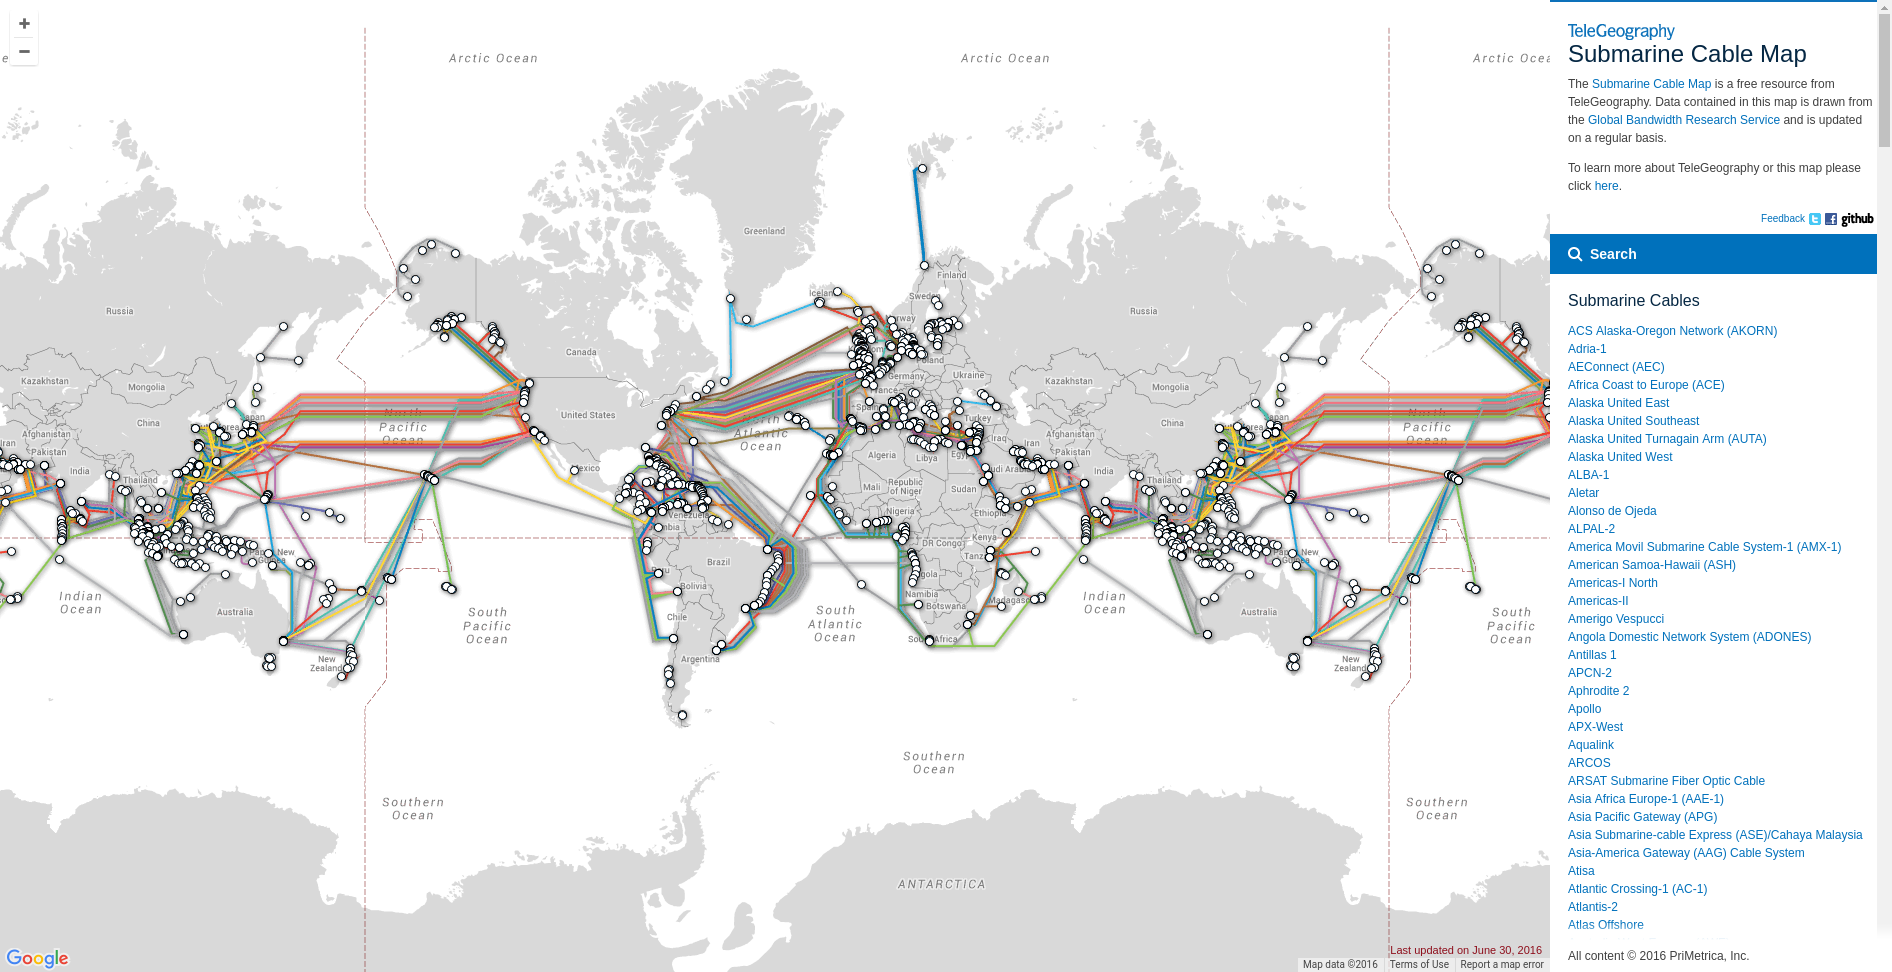
\includegraphics[width=\textwidth]{images/geovis/submarine.png}
    \caption[Overview of the submarine cable map]{Overview of the submarine cable map}
    \label{fig:submarine}
  \end{subfigure}
  \hfill
  \begin{subfigure}[b]{0.4\textwidth}
    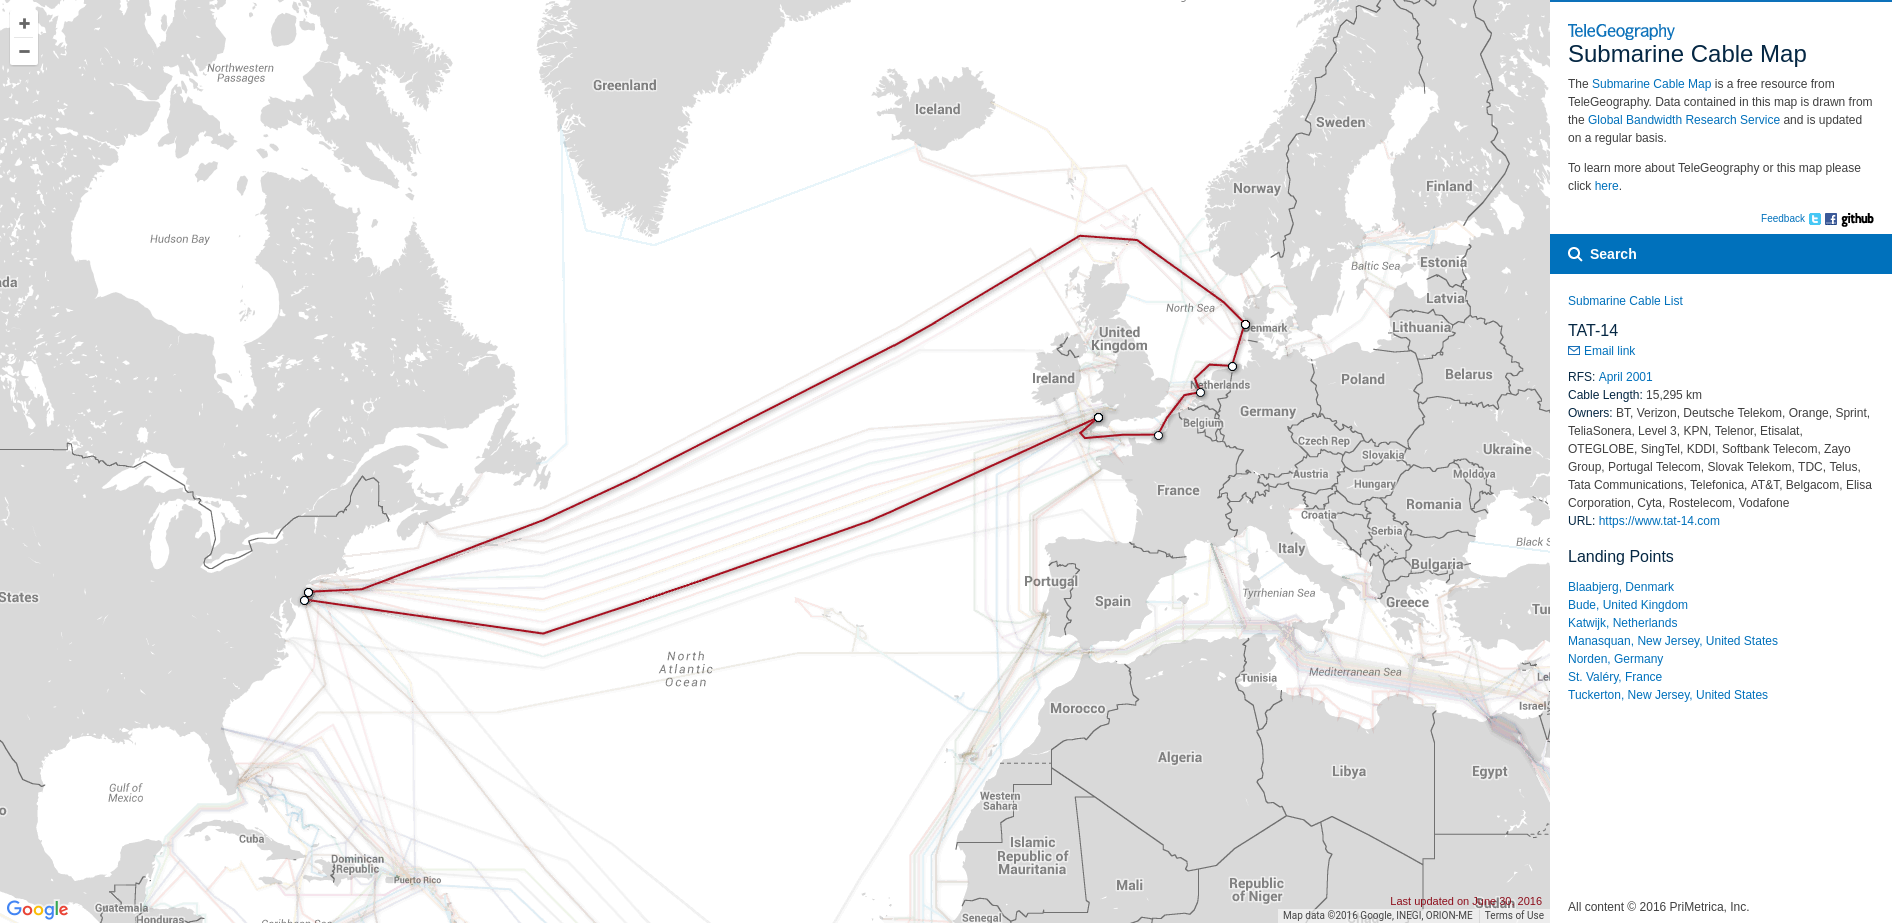
\includegraphics[width=\textwidth]{images/geovis/submarine-interactive.png}
    \caption[Interactivity of the submarine cable map]{Interactivity of the submarine cable map}
    \label{fig:submarine-interactive}
  \end{subfigure}
    \caption[
        TeleGeography’s free interactive submarine cable map, Urldate: 07.2016 \newline
    \small\texttt{\url{http://www.submarinecablemap.com/}}
    ]{TeleGeography’s free interactive submarine cable map}
  \label{fig:both-submarines}
\end{figure}

\item[E-commerce] \hfill \\
\ac{GeoVis} can be very useful in analysing data provided by e-commerce shops if they track orders-behaviour of their customers with some kind of geographical information. If such data is available and provided, it is possible to easily visualise the target group of a company on a map and therefore create knowledge and allow for generating hypothesis i.e. the next region for expansion.

\end{description}

\subsection{Interaction in visualizations}
\label{s:interaction}
When designing maps, there is one important distinction: designing maps for print versus the internet. For the first case, the design is for map readers, whereas for the latter case, it is for map users. The difference between readers and users lays in the interaction. This chapter focuses on a map designed for the internet and therefore allowing a lot more interaction. Users do not only interact but also manipulate web maps. Interaction for print maps would be moving a paper map closer or further away to one's eyes, or trim specific parts with scissors and so forth. The weakness of this kind of interaction is that the data on the map stays the same. However, zooming, selecting and moving a map on the internet actually allows for adapting the data shown \iacite{Muehlenhaus2014}.

As already mentioned in chapter \ref{s:definitions-types} on page \pageref{s:definitions-types}, \citeauthor{Shneiderman1996} published an often cited mantra \iacite{Shneiderman1996}:
\begin{quote}
"Overview first, zoom and filter, then details on demand."
\end{quote}

% MISSING BOOK: Information Visualization: Design for Interaction Spence 2007
% This mantra can also be used as a guideline for creating web maps with interaction.
% % Spence2007
% introduces a so called action cycle, which models an interactive exploration process of data. Small datasets, as well as complex and dynamic data can make use of this process in order to properly implement and integrate interaction.

% TODO - CHECK IF ENOUGH WORDS

The first part of this chapter will introduce some basic interaction methods and concepts. The second part will build upon the knowledge of the first part and maps the basic concepts to today's implementations with the focus on interaction with thematic maps.

\subsubsection{Overview First, Focus \& Context}
\input{chapters/methods/interaction/focus-context}

\subsubsection{Details on Demand}
\input{chapters/methods/interaction/dod}

\subsubsection{Multiple Views, Linking \& Brushing}
\label{s:linking-brushing}
\input{chapters/methods/interaction/linking}

\subsubsection{Animations and Transitions}
\input{chapters/methods/interaction/transition}




\subsection{State-of-the-art application analysis}
\section{Results}
\section{Discussion}
\section{Outlook}


\clearpage
% \addtocontents{toc}{\protect\pagebreak}
\begin{sloppypar}
\printbibliography
\end{sloppypar}
\iheader{References}

\clearpage
\listoffigures
\iheader{List of Figures}

\clearpage
\listoftables
\iheader{List of Tables}

% \clearpage
% \lstlistoflistings
% \iheader{List of Listings}


\setlength{\parskip}{10pt}
\end{document}